\documentclass{noithesis}

\newtheorem{theorem}{定理}[section]
\newtheorem{definition}[theorem]{定义}
\newtheorem{lemma}[theorem]{引理}
\newtheorem{property}{性质}[theorem]


\begin{document}
	
	\title{2023 程序设计 II 荣誉课程大作业报告}
	\author{中国人民大学~~李修羽}
	
	\maketitle
	
	\begin{abstract}
		本文主要探究了基于 Qt 图形界面应用设计的不围棋联网对战软件制作过程,对一些重要功能的实现进行了说明,同时对于团队分工过程有一定记录。在联网体系之外,额外探究了不围棋 AI 的算法设计与实现。
	\end{abstract}

	\tableofcontents
	\setcounter{page}{0}
	\thispagestyle{empty}
	\newpage
	
	\section{团队构成}
	
	\subsection{闲话}
	
	理论上这个大作业一个人也可以做,但是既然都称之为团队大作业了,那就团队做。
	
	\subsection{小组分工}
	
	笔者负责了项目 UI 的主要设计、棋盘逻辑的维护、文件部分的编写、AI 的设计与调试和报告的撰写。
	
	冯友和同学负责了项目框架的建构、联机部分的编写、项目的美化与调试和 AI 托管的实现。
	
	赵培宇同学负责了棋盘的生成、按钮的部分实现、状态的显示和对局重现的实现。
	
	\section{Qt 图形界面应用设计}
	
	\subsection{UI 设计}
	
	\begin{figure}[!htb]{
		\centering
		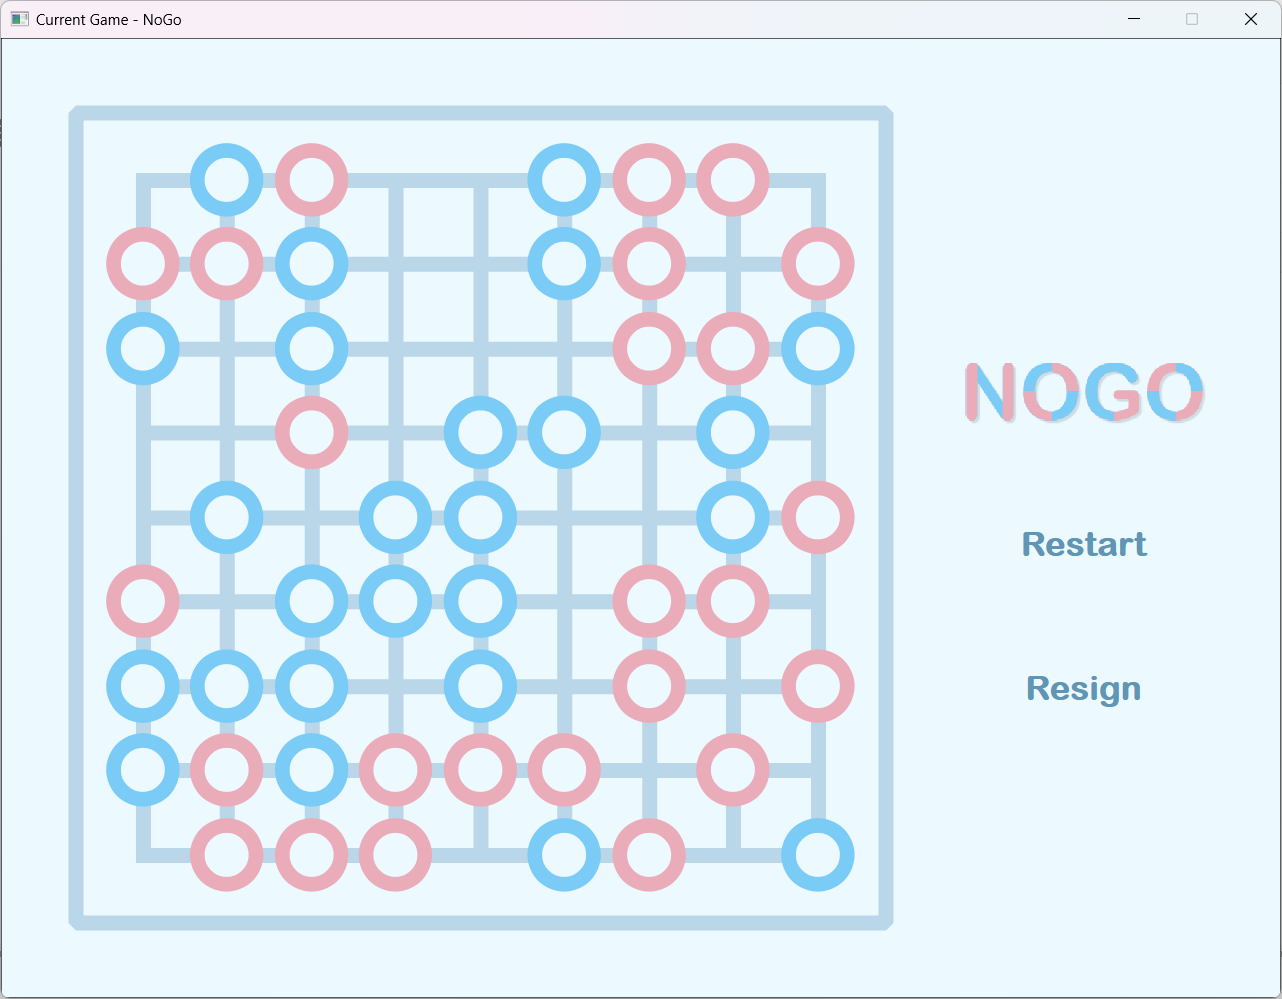
\includegraphics[width=0.8\textwidth]{img/UI.png}
		\counterwithin{figure}{subsection}
		\caption{demo 示例}
	}
	\end{figure}

	本应用 UI 设计\footnote{部分设计参考:https://github.com/epcm/QtNoGo}采用扁平化的设计风格,搭配上饱满、明亮、可爱且前卫的颜色设计,亮度统一且冷暖色调搭配,具有舒适的观感。字体使用 Sans-serif 字体 Arial Rounded MT Bold,平衡现代感和亲和感。棋子中心保留背景色,使棋盘整体更为协调。
	
	由于棋盘大小可以自定义,棋盘采用程序绘图而非图片覆盖的形式,可以根据棋盘的大小自适应调整棋盘线条粗细和棋子大小,保持程序页面分辨率相对不变。
	
	\begin{figure}[!htb]{
			\centering
			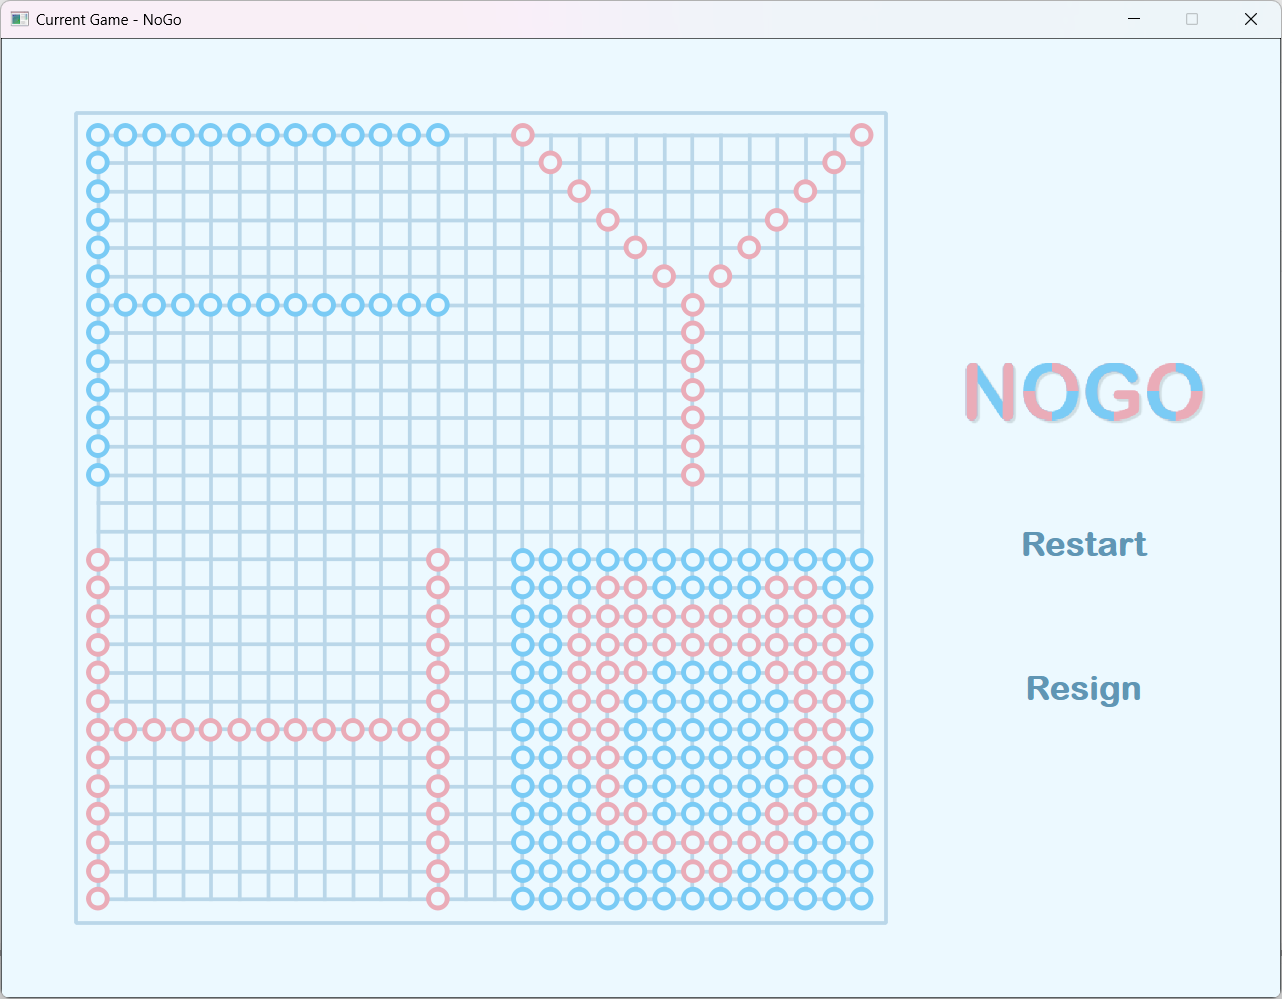
\includegraphics[width=0.8\textwidth]{img/fyh.png}
			\counterwithin{figure}{subsection}
			\caption{自定义棋盘大小~($28\times 28$)}
		}
	\end{figure}
	
	Logo 以棋子底色为设计基础,增加了颜色块的分割,具有棋类游戏的风格,也维持了项目的主要设计基调。

	\subsection{基本逻辑}
	
    \begin{verbatim}
|-- Qt-NoGo
    |-- DialogBox
    |   |-- messagebox.cpp
    |   |-- messagebox.h       // 弹出提示或结算信息
    |   |-- optiondialog.cpp
    |   |-- optiondialog.h     // 在联机对局时弹出申请窗口
    |   |-- optiondialog.ui
    |   |-- settingdialog.cpp
    |   |-- settingdialog.h    // 实现图形化更改游戏选项
    |   |-- settingdialog.ui
    |   |-- reviewdialog.cpp
    |   |-- reviewdialog.h     // 实现复盘功能
    |   |-- reviewdialog.ui
    |-- Object
    |   |-- bot.cpp
    |   |-- bot.h              // 随机下棋 bot
    |   |-- judge.cpp
    |   |-- judge.h            // 控制下棋过程逻辑,进程调度,局面判断
    |-- Resource.qrc           // 图片配置文件
    |-- Widget
    |   |-- gamewidget.cpp
    |   |-- gamewidget.h       // 维护对局棋盘状态,控制信号槽及文件读写
    |   |-- gamewidget.ui
    |   |-- startwidget.cpp    // 实现欢迎界面
    |   |-- startwidget.h
    |   |-- startwidget.ui
    |-- img                    // Logo 和 icon 图片
    |-- main.cpp
    |-- mynogo.pro             // QMake 项目管理文件
    |-- mynogo.pro.user
    |-- network                // 网络库相关
    |   |-- networkdata.cpp
    |   |-- networkdata.h
    |   |-- networkserver.cpp
    |   |-- networkserver.h
    |   |-- networksocket.cpp
    |   |-- networksocket.h
    |-- report                 // 项目报告
	\end{verbatim}

	基本逻辑为 \verb|main| 连接信号槽后切换到 \verb|startwidget|,通过 \verb|optiondialog| 设置后进入 \verb|gamewidget|,由 \verb|gamewidget| 初始化 \verb|judge| 开始游戏。游戏过程由 \verb|judge| 判断,发现终局后传输到 \verb|gamewidget| 然后输出 \verb|messagebox| 信息,至此一局游戏结束。

	\subsection{棋盘逻辑和结局判断}
	
	由于最后 NoGo-Cup 给 AI 的限时是 $3s$,留给 AI 计算的时间并不充裕,所以本项目采用了高效率的棋盘底层逻辑,以期为 AI 的运行提供尽可能多的时间。
	
	相较于传统的 dfs 判断棋子,笔者创新性地采用了启发式合并的方法来判断棋子的连通性与气数,在 \verb|judge.h| 中的定义如下:
	
	\begin{lstlisting}
	typedef std::pair<int, int> Item;
	typedef std::vector<Item> ItemVector;
	typedef std::set<Item> LibertySet;

	int board[CHESSBOARD_SIZE + 2][CHESSBOARD_SIZE + 2]; // 当前棋盘状态
	int chessBelong[CHESSBOARD_SIZE + 2][CHESSBOARD_SIZE + 2]; // 棋子属于的棋子块
	int blockVis[(CHESSBOARD_SIZE + 2) * (CHESSBOARD_SIZE + 2)]; // 棋子块至多只能累加一次
	int blockCnt; // 棋子块个数
	
	LibertySet blockLiberty[(CHESSBOARD_SIZE + 2) * (CHESSBOARD_SIZE + 2)]; // 气的 Set
	ItemVector chessBlock[(CHESSBOARD_SIZE + 2) * (CHESSBOARD_SIZE + 2)]; // 棋子块的编号
	std::vector<int>mergedBlock;
	\end{lstlisting}

	本程序用 \verb|vector| 存储每一个连通块棋子的位置,用 \verb|set| 存储每一个连通块气的位置。对于一次合并,将两端连通块的 \verb|vector| 和 \verb|set| 分别启发式合并即可。此处采用 \verb|set| 是因为其本身具有判重的特性,可以在合并时对气做出高效率的处理。
	
	\begin{lstlisting}
		
	void Judge::MergeSet(LibertySet &x, LibertySet y)
	{
		if(x.size() < y.size()) std::swap(x, y);
		for(Item u : y) x.insert(u);
	}
	void Judge::MergeBlock(int x, int y) // 启发式合并
	{
		if(chessBlock[x].size() < chessBlock[y].size()) std::swap(x, y);
		MergeSet(blockLiberty[x], blockLiberty[y]);
		for(Item u : chessBlock[y])
		{
			chessBlock[x].push_back(u);
			chessBelong[u.first][u.second] = x;
		} // 合并
		chessBlock[y].clear(); // 清空
	}
	\end{lstlisting}

	相较于 dfs 判断单次 $O\left(n^2\right)$ 的复杂度,启发式合并的复杂度可以做到 $O\left(\log^2 n\right)$,且此处的 $n^2$ 仅为理论上界,对于大规模棋盘(例如 $20\times 20$)有极高的效率。
	
	对于一次落子操作,如果落子后判负,会弹出此处无法落子的弹窗。同时在一次操作超时后,会直接超时判负。对于现有版本来说,页面实现了认输按钮,玩家在无法落子后可以等到超时判负,也可以认输判负。
	
	\begin{figure}[htbp]
		\centering
		
		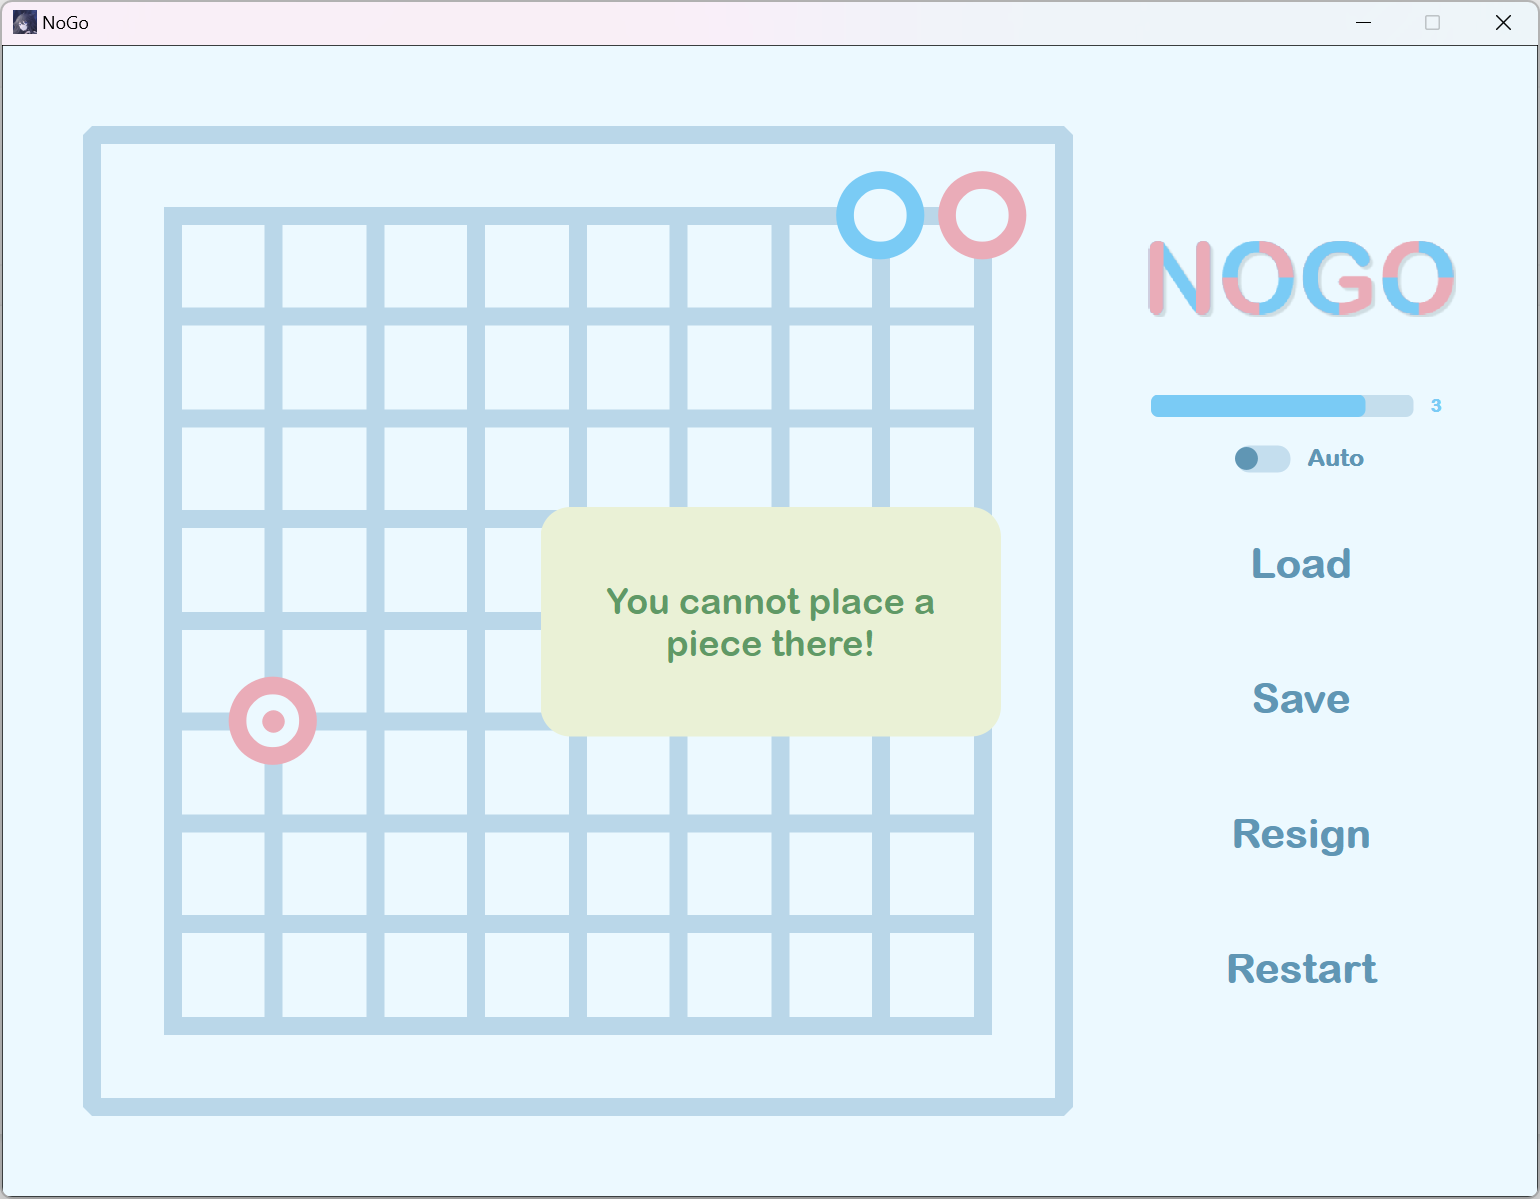
\includegraphics[width=5.5cm]{img/tip.png}	
		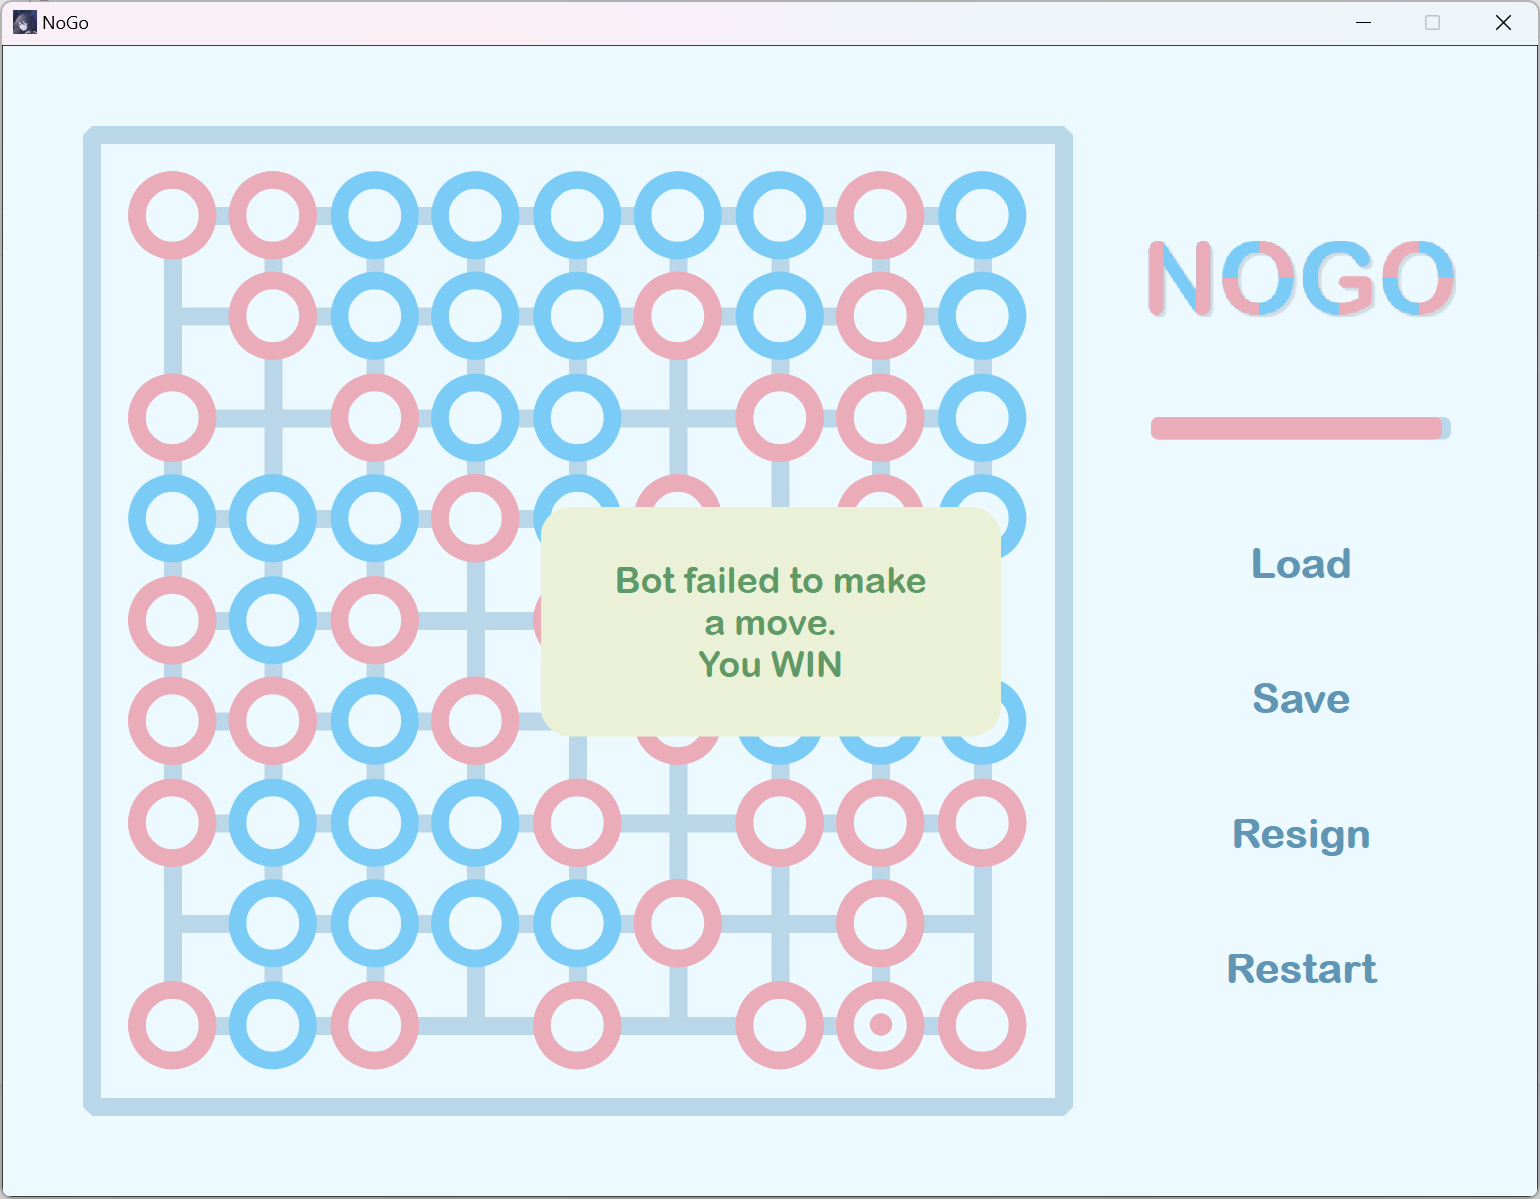
\includegraphics[width=5.5cm]{img/win.png}
		
		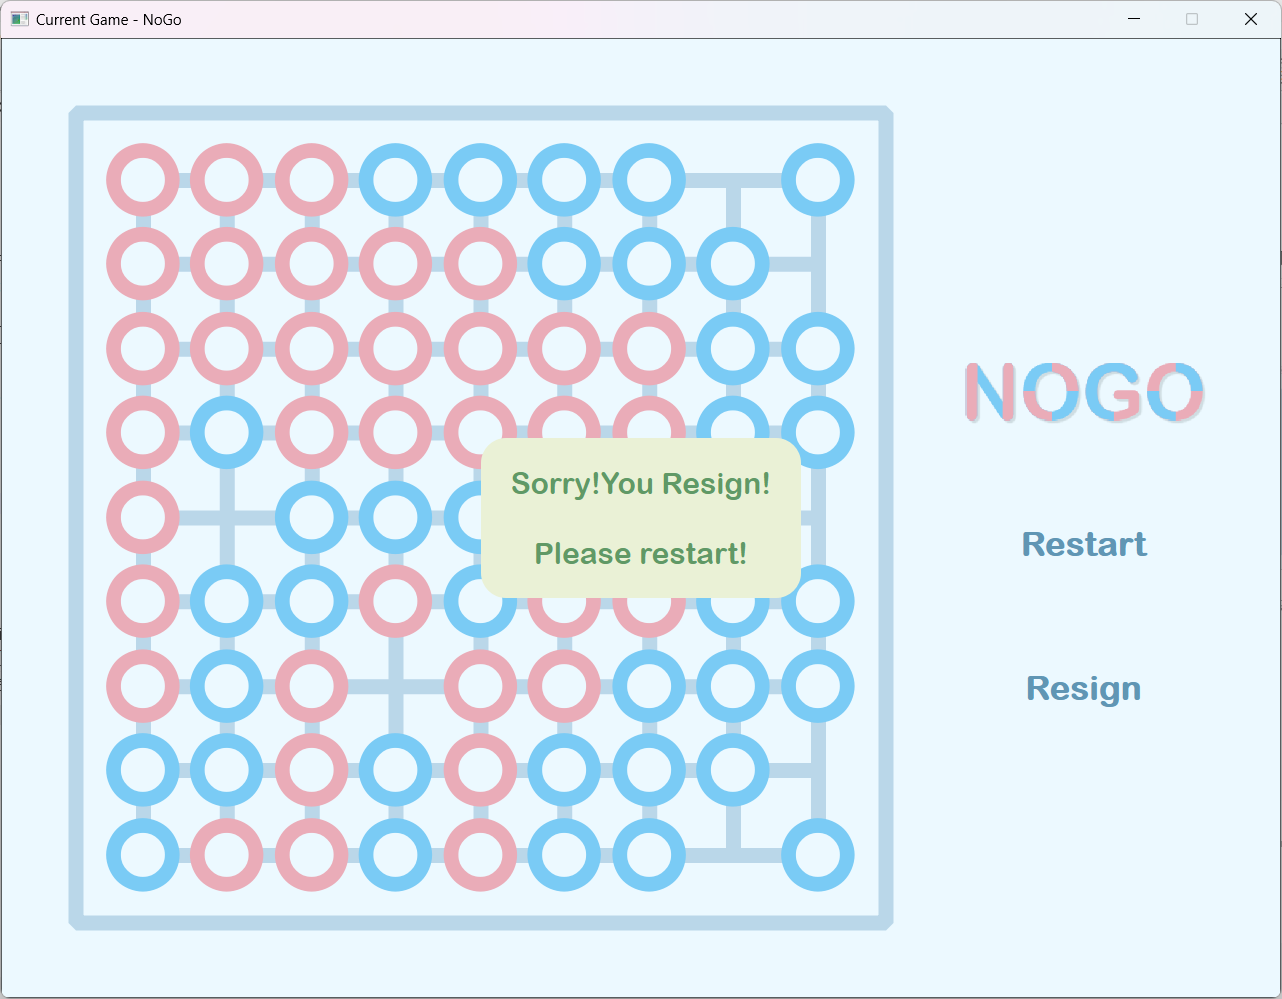
\includegraphics[width=5.5cm]{img/resign.png}
		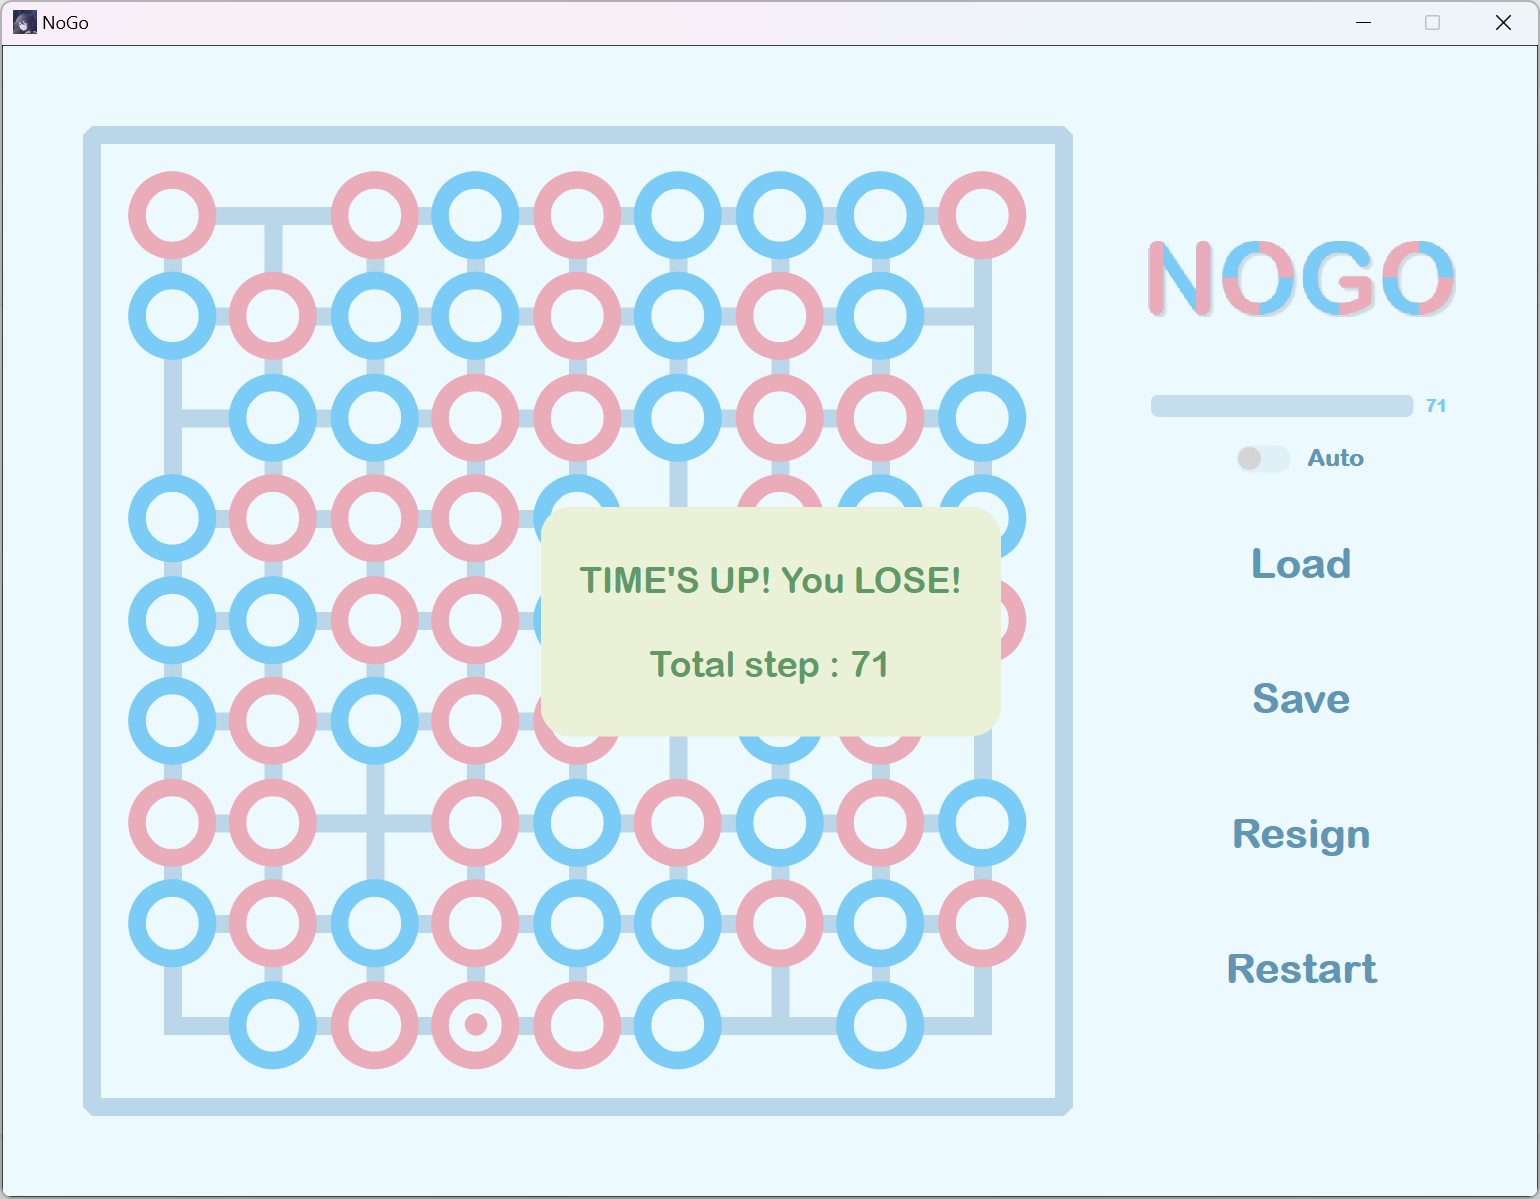
\includegraphics[width=5.5cm]{img/TLE.png}
		
		\counterwithin{figure}{subsection}
		\caption{状态判断}
	\end{figure}
	
	但是在后期 AI 的实现过程中,笔者发现该算法实现回退搜索树(可持久化数组)的时空代价太大。所以在 AI 计算时,我们单独从 \verb|judge| 中取出状态数组进行 dfs 判断,非本地 AI 操作和终局回放仍使用原逻辑,这样实现的耦合度也较低。
	
	\subsection{设置}
	
	设置部分基于 \verb|optiondialog| 类,使用 Qt 自带的文本选择框和按钮对 \verb|gamewidget| 传入棋盘大小、游戏模式和联机部分的信息,将在线与离线、PVP 与 PVE 利用有限的空间优秀地集成为一体,用按钮切换在线模式与离线模式。
	
	在线模式下,参数采用统一的 $9\times 9$ 棋盘大小。
		
	\begin{figure}[!htb]{
			\centering
			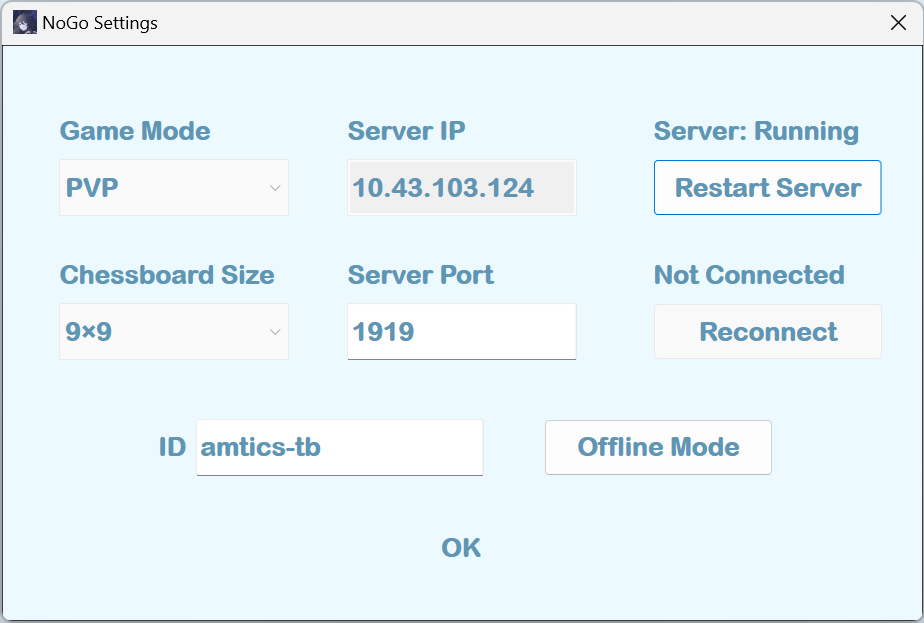
\includegraphics[width=8cm]{img/web1.png}
			\counterwithin{figure}{subsection}
			\caption{设置页面}
		}
	\end{figure}
	
	\subsection{计时器和状态显示}
	
	计时器基于 \verb|QProgressBar| 自带的 \verb|TimeBar|,用 CSS 设置美化后用于本项目的计时器设计。计时器采用从右向左线性读条的方法计时,进度条结束后判定为超时。
	
	状态显示位于计时器右侧,可以显示当前总步数。
	
	在终局(胜利、失败、认输)后,计时器会与棋盘本体一起冻结,在对局重现时会随着 Try 的介入而重新启用。
	
	\subsection{读档和存档}
	
	项目将棋盘的每一步存入 \verb|vector| 中,并编码为形如 \verb|0/2 0/1 A1 B4 D3 G/W/L| 的字符串形式存入 \verb|DATA(.dat)| 文件中。第一个数字 \verb|0| 代表执黑、\verb|2| 代表执白,第二个数字 \verb|0| 代表 PVP、\verb|1| 代表 PVE,最后的字符 \verb|G/W/L| 代表认输/胜利/失败。
	
	文件操作基于 \verb|QFile| 和 \verb|QFileDialog| 实现,\verb|QFileDialog::getSaveFileName| 可以实现打开文件框保存文件,\verb|QFileDialog::getOpenFileName| 可以实现打开文件框读取文件。文件流使用 \verb|QFile::readAll| 和 \verb|QFile::write|,传输类型为 \verb|QByteArray| 与 \verb|char*|。
	
	以下是存档部分的实现:
	
	\begin{lstlisting}
	// 存档按钮信号
	void GameWidget::on_saveButton_clicked()
	{
		dataToString(); // 将数据编码到 char* dataStr 中
		QString fileName = QFileDialog::getSaveFileName(nullptr, tr("Save Data"), "", tr("DATA (*.dat)"));
		// QFileDialog 读取文件 fileName
		if (fileName.isEmpty())
			return;
		else
		{
			QFile file(fileName);
			if (!file.open(QIODevice::WriteOnly)) // 无法覆写时报错
			{
				QMessageBox::information(nullptr, tr("Unable to open file"),file.errorString());
				return;
			}
			file.write(dataStr); // QFile 直接读写文件
			file.close();
		}
	}
	\end{lstlisting}
	
	读档后,程序重新初始化棋盘,强制传入存档内的设置参数,顺序模拟所有下棋操作。操作完成后得到的便是 Save 时的游戏状态,读档后 \verb|TimeBar| 重置为初始时间,如果不是终局仍可以继续下棋,并随时可以执行新的 Save 和 Load。
	
	\subsection{信息窗口}
	
	\verb|messagebox| 类实现了页面内的弹出信息,下棋界面内的信息包括自杀的濒死检测和游戏终局的判断。
	
	信息窗口会一直显示到检测鼠标单击,而对于终局显示的信息窗口,至少显示 $3s$ 后才能关闭。
	
	\subsection{更多功能}

	\subsubsection{附加任务 1,2 实现}
	
	附加任务:
	
	1. 在重现对局中实现播放,暂停,上一步,下一步,到第\_步 等功能。
	
	2. 重播对局时可以随时介入进行不一样的尝试,尝试后也可以还原并继续播放。
	
	这两个附加功能主要通过 \verb|reviewdialog| 实现。当使用者在使用 Load 功能时,如果 Load 的文件显示保存的对局是已经结束的完整对局,我们便会弹出 \verb|reviewdialog| 窗口,进入复盘模式。
    在复盘模式下我们可以通过按钮点击的方式,实现对局自动播放、暂停、上一步、下一步、介入尝试、退出尝试功能,通过输入数字的方式实现跳转到指定步数功能。
  
    接下来将逐一介绍各个功能的实现。
    
    \verb|reviewdialog| \textbf{类设计}
    
    \begin{lstlisting}
    	// 存档按钮信号
	class ReviewDialog : public QDialog {
		Q_OBJECT
		public:
			explicit ReviewDialog(Judge *pjudge,QWidget *parent = nullptr);
			~ReviewDialog();
			void set_review_data(char state,char data[],ItemVector v);
			void init();
		signals:
			void trybutton(); 
			void quit_try();
		public slots:
			void display();    
			private slots:
			void on_start_clicked();	
			void on_pause_clicked();
			void on_previous_clicked();
			void on_next_clicked();
			void on_tryButton_clicked();
			void on_quit_try_clicked();
			void on_input_entered();
		private:
			void paintEvent(QPaintEvent *event) override;
			Ui::ReviewDialog *ui;
			int WIDTH=687, HEIGHT=204;  //dialog 大小
			MessageBox *messagebox;
			Judge *judge;
			char strState; 
			char dataStr[28 * 28 * 3 + 5];
			ItemVector dataVec;		//储存对局信息的vector
			int sum_steps;  //总共有多少步
			QTimer *tim;    //自动播放的计时器
			int now_step = 0;   //当前进行到哪一步
	};
    \end{lstlisting}
    
    \textbf{播放与暂停}
    
    我们使用 \verb|Qtimer| 来控制自动播放,当按下播放按钮时,\verb|Qtimer| 开始运行,每隔 $0.5s$ 进行一步,通过变量 \verb|now_step| 的实时更新读取 \verb|datavec[now_step]| 数据,实现自动播放。当按下暂停按钮时,使 \verb|Qtimer| 暂停,从而实现暂停播放。
    
	\textbf{上一步/下一步}
	
	当按下上一步或下一步按钮时,首先执行暂停操作,之后变量 \verb|now_step| 会相应的加一或减一,从而实现上下步的变换。

	\textbf{跳转到第\_步}
	
	通过 \verb|Qlineedit| 读取到用户输入的文本,执行暂停操作后,将读取到的数字赋值给 \verb|now_step|,从而实现跳转指定步数。
	
	\textbf{介入尝试与退出尝试}
	
	当用户点击 Try 按钮时,原本被锁定的棋盘解锁,同时其他按钮除退出尝试外均被禁用。
	
	用户可以通过鼠标点击实现落子,不可再打开 Auto 模式,同时会根据 Load 的 \verb|data| 来判断对局是 PVP 还是 PVE。
	
	当用户点击 Quit Try 按钮时,棋盘会锁定,其他按钮被启用,同时通过之前储存的 \verb|now_step| 跳转到 Try 之前的局面。
	
	\begin{figure}[htbp]
		\centering
		
		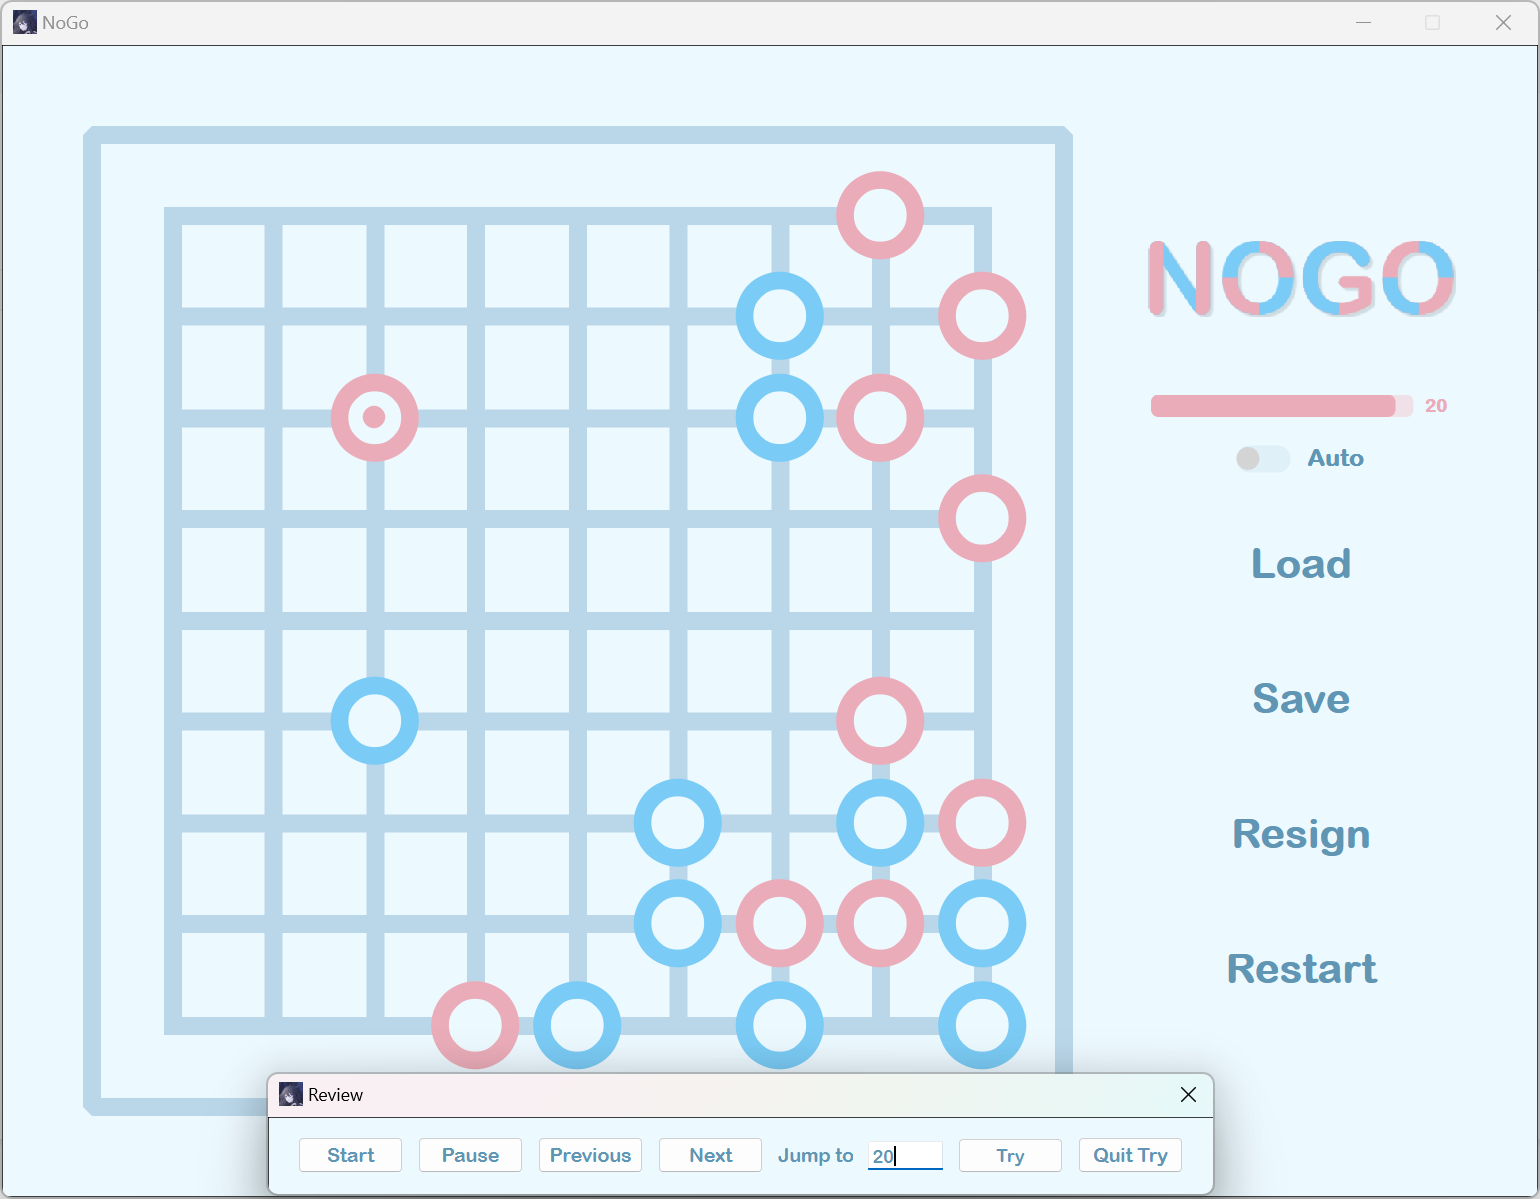
\includegraphics[width=5.5cm]{img/review1.png}	
		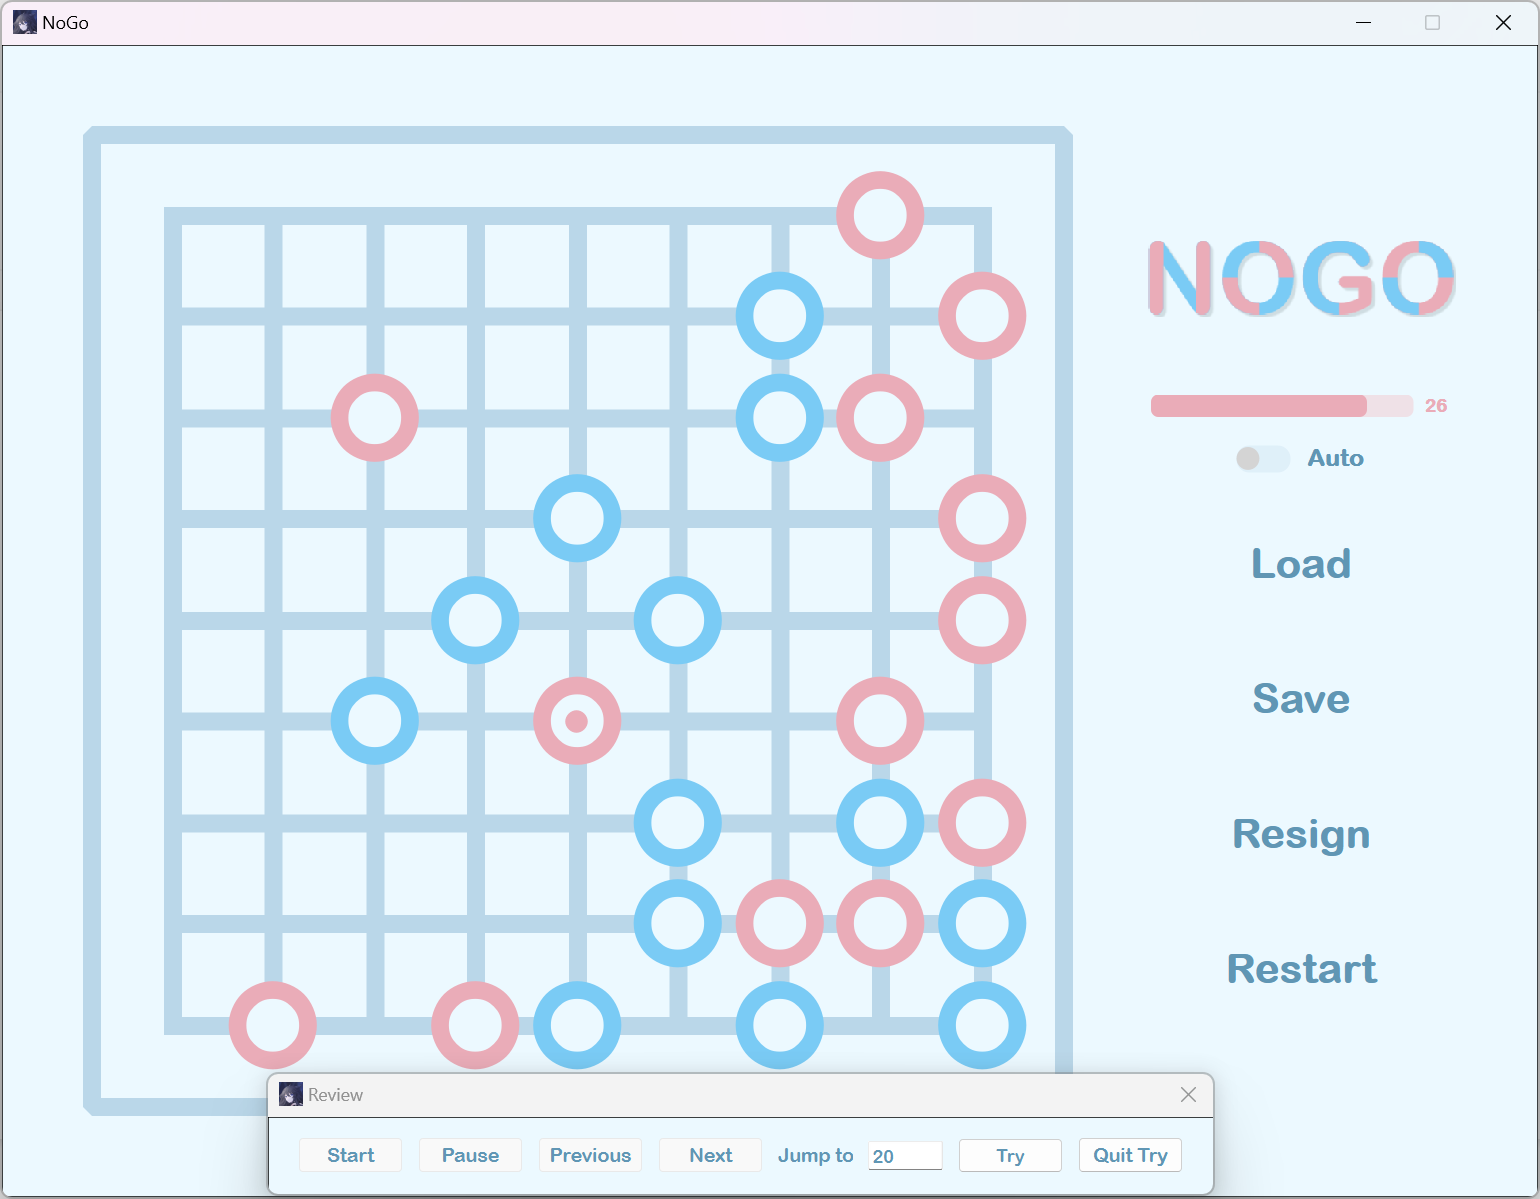
\includegraphics[width=5.5cm]{img/review2.png}
		
		\counterwithin{figure}{subsection}
		\caption{对局重现}
	\end{figure}

	\subsubsection{其他功能}
	
	没有写更多功能是怎么回事呢?大作业相信大家很熟悉,但是没有写更多功能是怎么回事呢?笔者也不是很清楚,大家也可能感到很惊讶,没有写更多功能是怎么回事呢?但事实就是这样,可以前往 \href{https://ce-amtic.github.io/}{ce-amtic 的博客} 看博客。
	
	\sout{哦,应该是 duality314 比较摆烂没写,记得去 push。}
	
	duality314 写完了该 push ce-amtic 了。
	
	\section{联机对战设计}
	
	\subsection{通信协议}
	
	联机功能使用基于 \verb|QTcpServer, QTcpSocket| 二次封装的 \verb|NetworkServer, NetworkSocket| 类实现,可以通过 TCP 协议进行同一局域网内两个终端点对点的数据交换。
	
	联机传输的数据通过 \verb|NetworkData| 类进行封装,数据类型如下:
	\begin{lstlisting}
	enum class OPCODE : int {
    	READY_OP = 200000,  // 申请对局
    	REJECT_OP,          // 拒绝对局
	    MOVE_OP,            // 一方落子
	    GIVEUP_OP,          // 一方认输
	    TIMEOUT_END_OP,     // 结算,终局条件为一方超时未落子
	    GIVEUP_END_OP,      // 结算,终局条件为一方认输
	    LEAVE_OP,           // 一方断开连接
	    CHAT_OP,            // 进行聊天数据交换
	};
	\end{lstlisting}

    \subsection{联机对战逻辑}
    
    进行一场联机对战可以抽象为以下三个步骤:1.双方建立连接;2.一方发起对局,另一方确认对局;3.完成对局并确认胜负,返回第一步结束后的状态。
	
	\subsubsection{双方建立连接}
	
	首先在设置 UI 中加入 IP、端口、用户昵称的输入框,以获取必要的信息。然后在数据库 \verb|Judge| 类中创建 \verb|(NetworkServer*)server, (NetworkSocket*)socket| 对象,在构造函数中初始化,用于建立连接。
	
	在设置 UI 中加入 启动服务器(Restart Server) 与 连接服务器(Reconnect) 的按钮,行为如下:当 Restart Server 按钮被点击时,调用 \verb|QTcpServer::listen(port)| API 来监听用户所输入的端口;当 Reconnect 按钮被点击时,调用 \verb|NetworkSocket::hello(host, port)| API 来尝试与地址为 \verb|host:port| 的主机通信。
	
	调用 \verb|QTcpSocket::waitForConnected()| API 来判断是否连接超时,若超时则提示未连接并禁止用户发起对局,否则提示连接正常并等待下一步。
	
	\subsubsection{一方发起对局,另一方确认对局}
	
	当 Restart Server 和 Reconnect 按钮中有一者被点击时,视作应用程序进入了联机模式。在联机模式下,点击对局开始按钮并不会立刻跳转到棋盘界面,而是会弹出 \verb|OptionDialog| 类所创建的提示窗口,提示等待连接。其中 \verb|OptionDialog| 类基于 \verb|QDialog| 类二次封装,并进行了一些美化。
	
	此时,提出邀请发发送 \verb|READY_OP| 型数据,接收方识别该数据,并弹出同样的 \verb|OptionDialog| 来确认对局是否成立,返回 \verb|READY_OP| 或 \verb|REJECT_OP|。
	
	当对局成立时,双方同时进入棋盘界面,否则返回第一步结束后的状态。 

    \subsubsection{完成对局并确认胜负}
    
    对局成立后执黑先行。对于当前落子一方,每次落子成立时均会向对方发送 \verb|MOVE_OP| 信号,并结束监听鼠标点击。对方接受 \verb|MOVE_OP| 信号后会绘制该棋子,并开始监听己方鼠标点击。
    
    在对局中,双方可以通过界面右下的聊天框进行实时沟通,通过互相发送 \verb|CHAT_OP| 实现。
    
   \begin{figure}[!htb]
    	\centering
    	
    	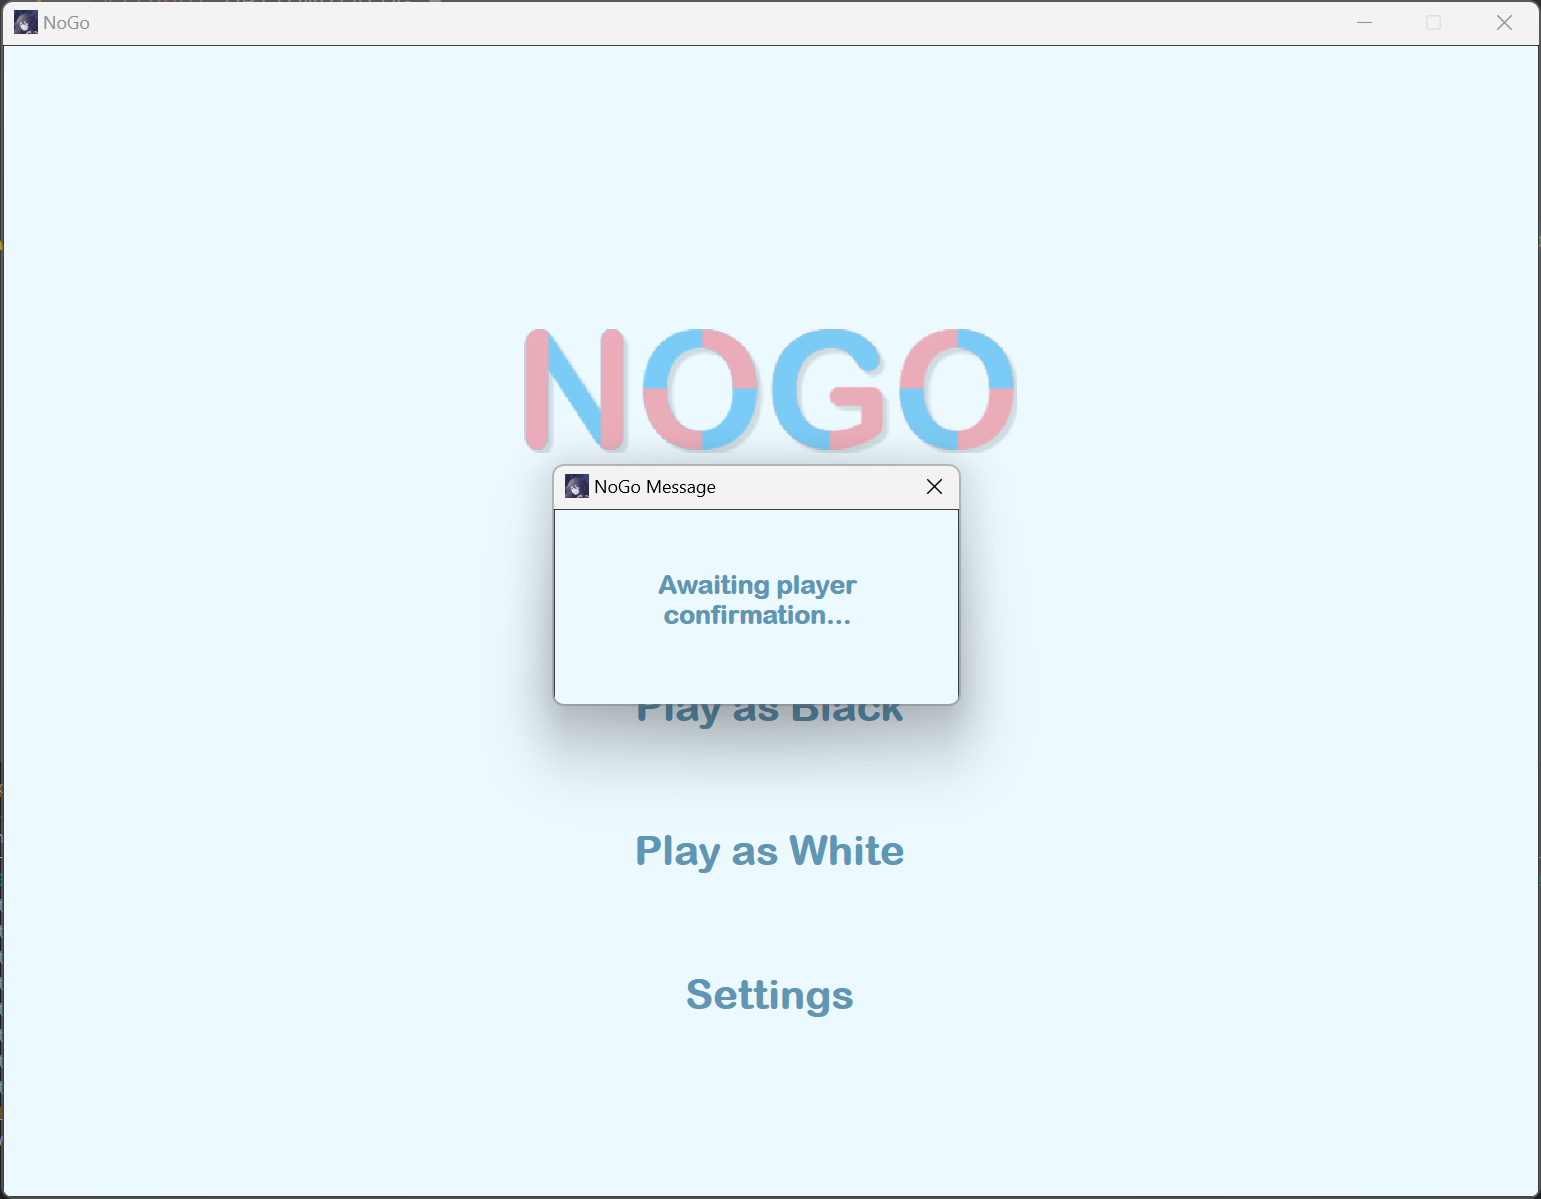
\includegraphics[width=5.5cm]{img/web4.png}
    	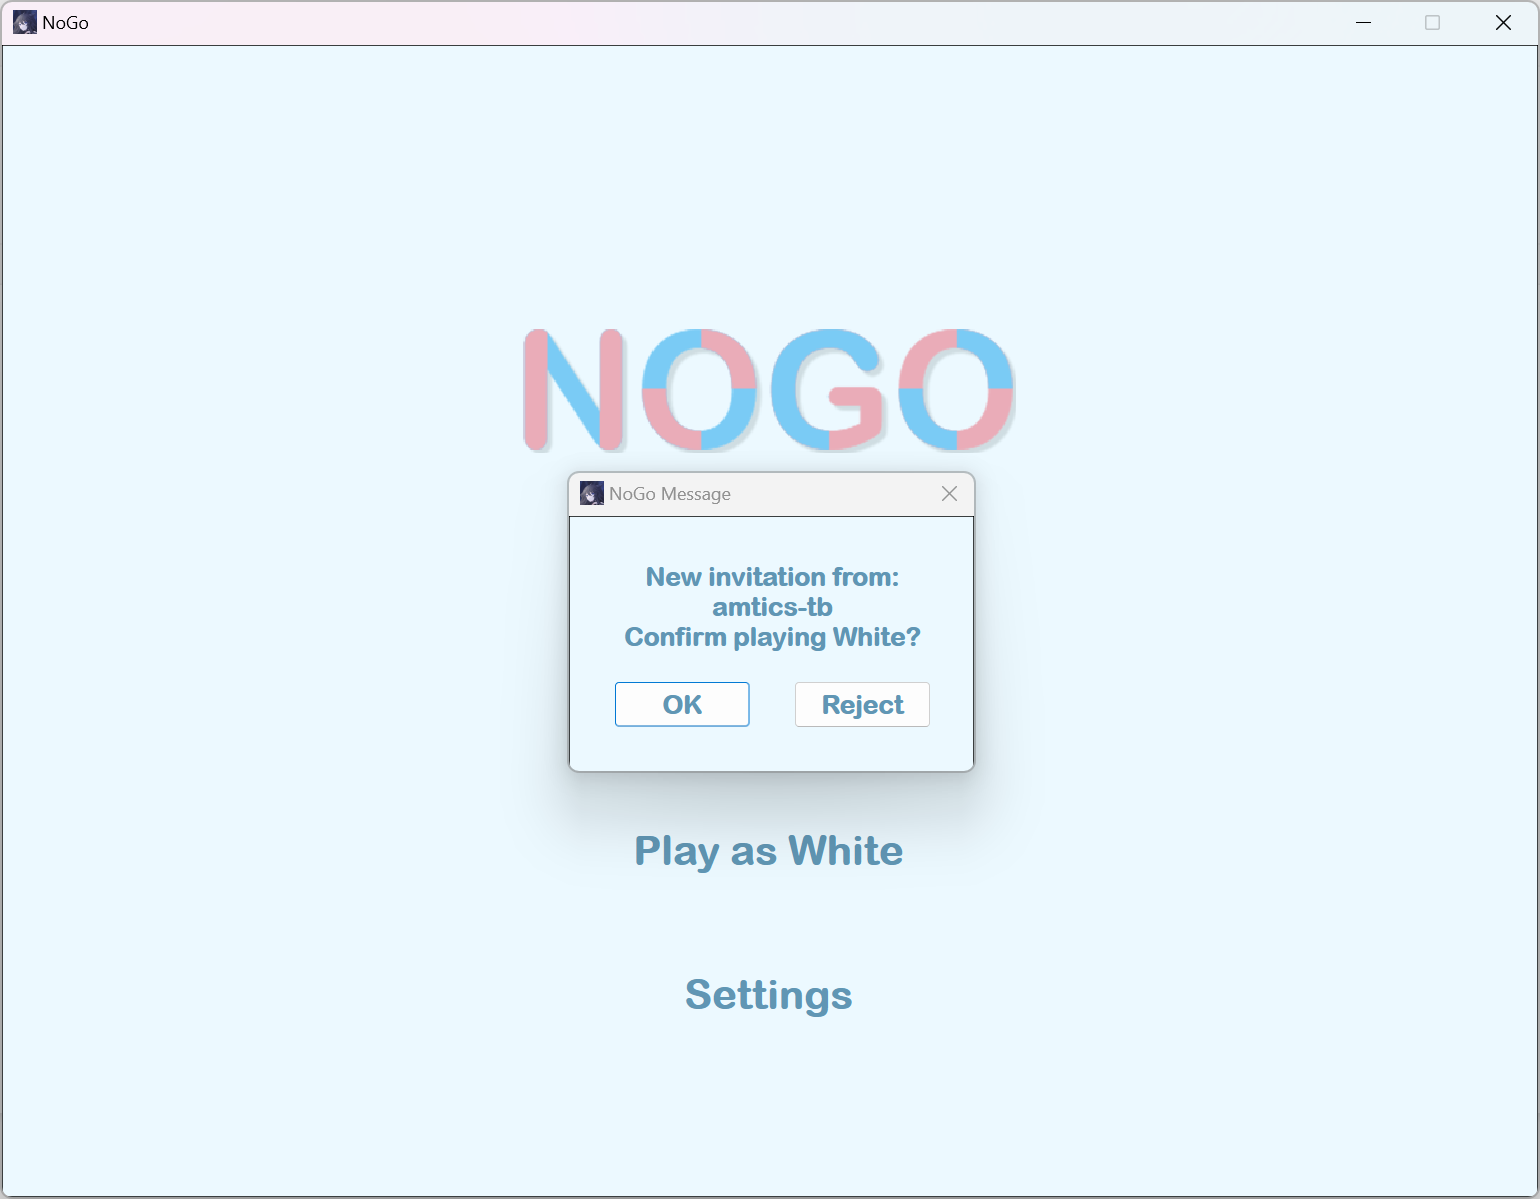
\includegraphics[width=5.5cm]{img/web5.png}
    	
    	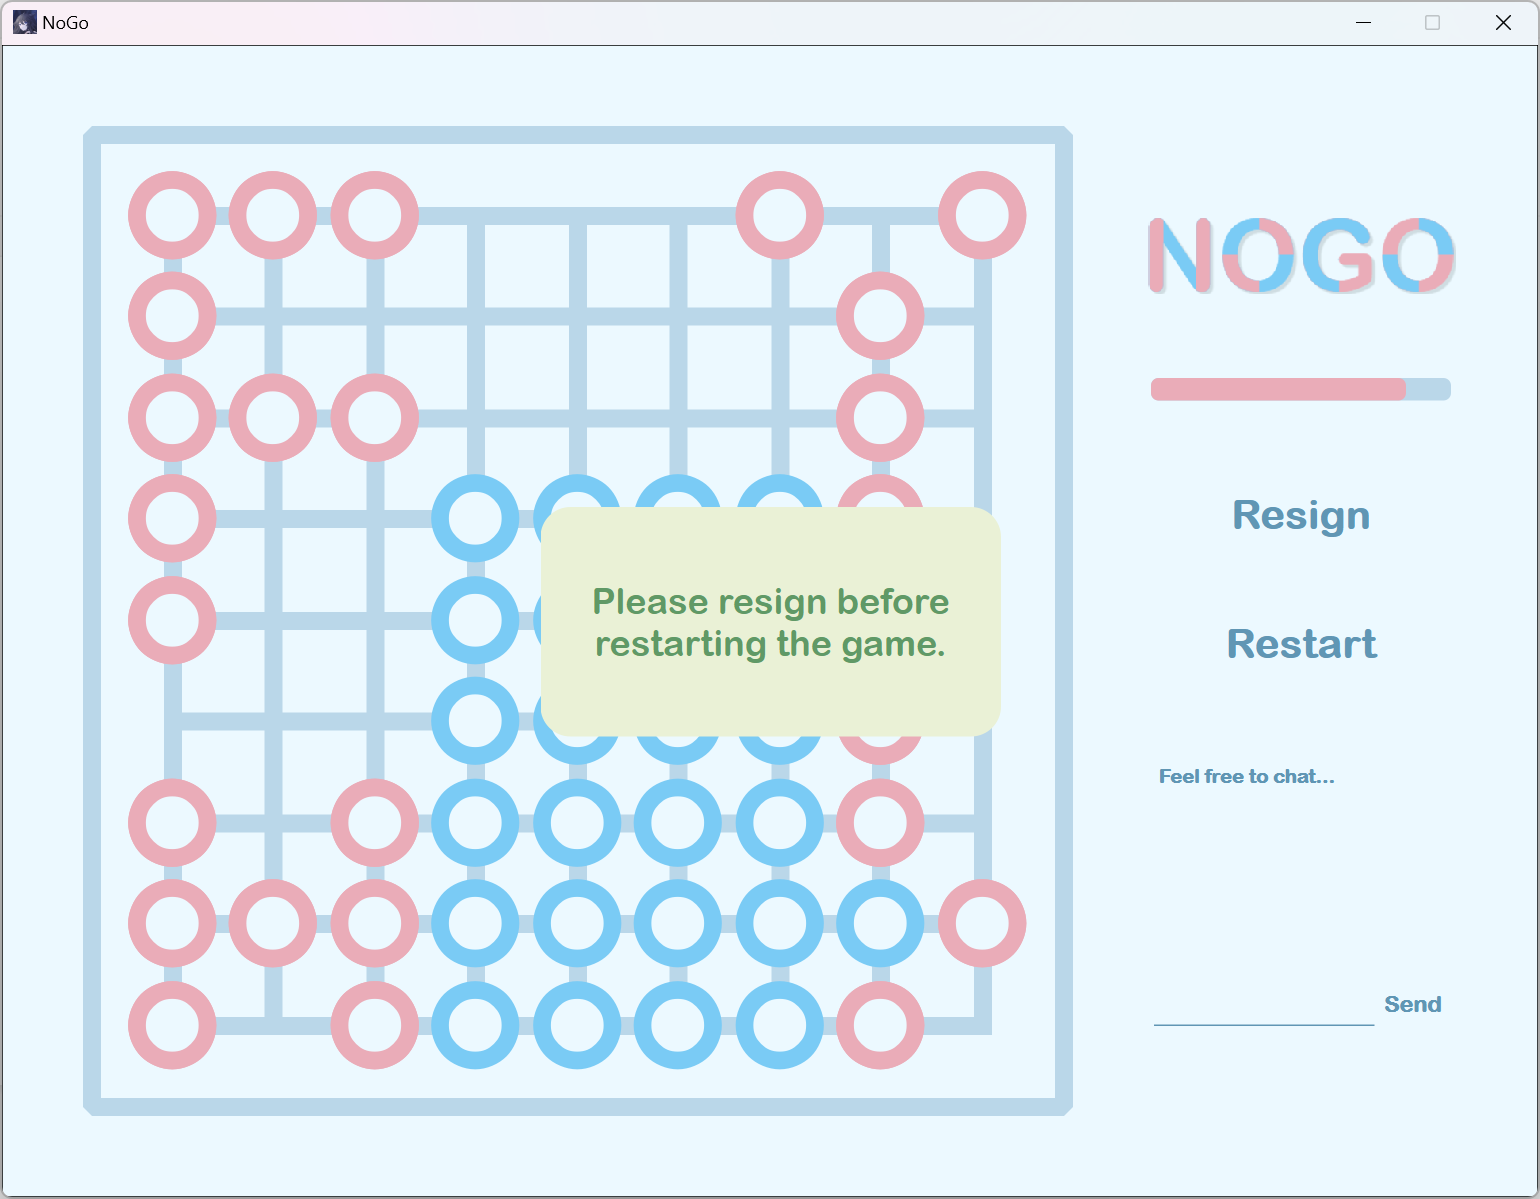
\includegraphics[width=5.5cm]{img/web2.png}
    	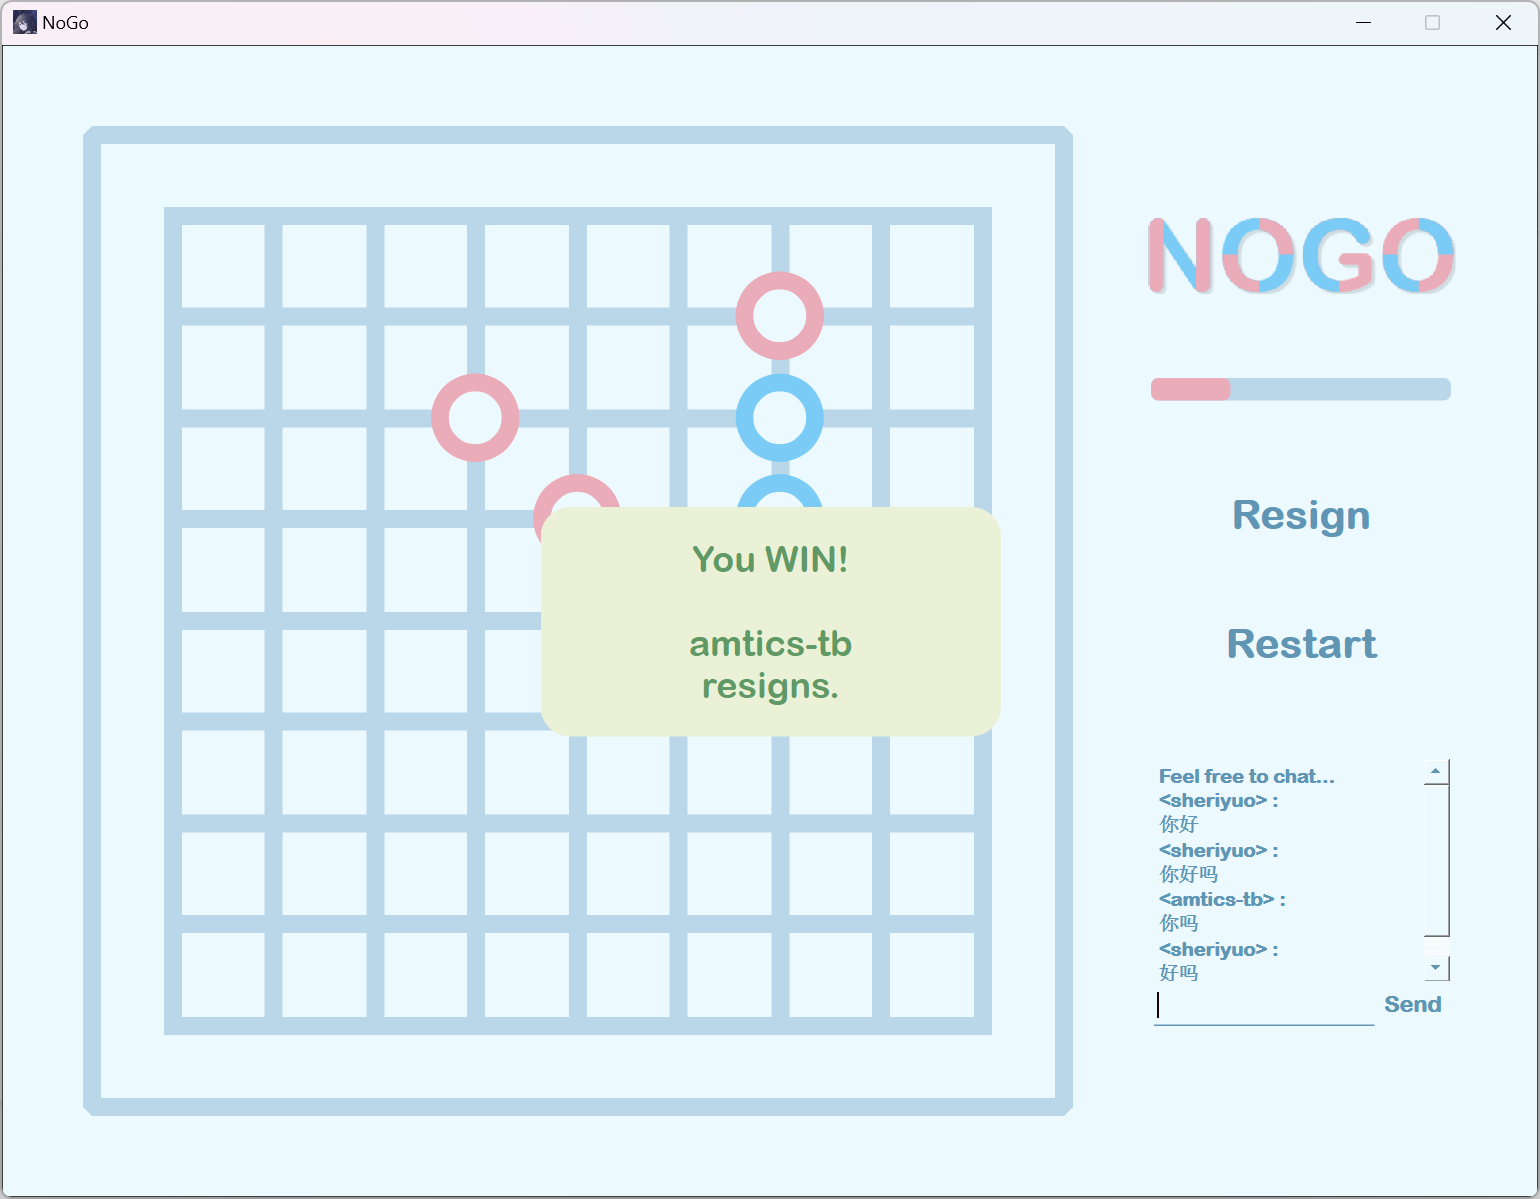
\includegraphics[width=5.5cm]{img/web3.png}
    	
    	\counterwithin{figure}{subsection}
    	\caption{联机对局界面演示}
    \end{figure}
    
    由于在判断落子成立时禁止了棋手自杀,因此对局结束的条件只有超时和认输两种。
    
    当一方认输,即点击 Resign 按钮后,认输方发送 \verb|GIVEUP_OP|,胜方在收到该信息后回复 \verb|GIVEUP_END_OP| 表示请求以“一方认输”为理由结束对局。认输方收到 \verb|GIVEUP_END_OP| 回复同样的信息以确认。此时联机对战结束,棋盘不能被操作。
    
    当一方超时,胜方的计时器会调用 \verb|GameWidget::playerTimeout_OL()| 槽函数,发送 \verb|TIMEOUT_END_OP| 表示请求以“一方超时”为理由结束对局,负方回复同样的信息以确认。此时联机对战结束,棋盘不能被操作。
    
    当联机对战结束时,对局双方可以分别选择是否返回开始界面。当双方都返回开始界面后,此时程序视作重置到了第一步完成后的状态,可以选择重新开始联机或单人对局。
    

	\section{AI 算法设计}
	
	由于助教在 \verb|/guidance| 中建议不要卷 AI 的强度,所以本项目 AI 采用推荐的 Minimax 搜索算法。
	
	同时,对于用 MCTS 爆杀本项目 AI 的隔壁队伍表示强烈的谴责。
	
	\subsection{Minimax 搜索和 Alpha-Beta 剪枝}
	
	Minimax 算法又叫极小化极大算法,是一种找出失败的最大可能性中的最小值的算法。
	
	Minimax 算法的整个过程,会从上到下遍历搜索树,回溯时利用子树信息更新答案,最后得到根节点的值,意义就是我方在双方都采取最优策略下能获得的最大分数\footnote{摘选自:https://oi-wiki.org/search/alpha-beta/}。
	
	Alpha-Beta 剪枝为每一个节点确定分数区间 $[\alpha, \beta]$,当 $\alpha \geq \beta$ 时停止搜索。
	
	代码框架如下:
	
	\begin{lstlisting}

// minimax 搜索
double Bot::alphaBeta(double a, double b, int depth)
{
	time_t curTime = clock();
	if((curTime - searchStartTime) / (BOT_TIMEOUT * 1000) > 0.9)
		return depth & 1 ? b : a; // 判断超时
	if(depth == Max_Dep)
		return judgeBoard(); // 叶子节点返回估价
	if(depth & 1)
	{
		int op = 0;
		for(auto [xx, yy] : chooseVec)
			if(checkBoard(xx, yy)) // 枚举搜索节点 (xx, yy)
			{
				op = 1;
				/* 更新状态 */
				b = std::min(b, alphaBeta(a, b, depth + 1));
				/* 回溯状态 */
				if(a >= b) 
					break;
			}
		if(!op)
			return judgeBoard(); // 叶子节点返回估价
		return b;
	}
	else
	{
		int op = 0;
		for(auto [xx, yy] : chooseVec)
			if(checkBoard(xx, yy)) // 枚举搜索节点 (xx, yy)
			{
				op = 1;
				/* 更新状态 */
				a = std::max(a, alphaBeta(a, b, depth + 1));
				/* 回溯状态 */
				if(depth == 0 && /* 更优 */ )
				{
					/* 更新状态 */
				}
				if(a >= b) 
					break;
			}
		if(!op) 
			return judgeBoard(); // 叶子节点返回估价
		return a;
	}
}
	\end{lstlisting}
	
	其中,\verb|chooseVec| 为随机排序的存储空位的 \verb|vector|,\verb|judgeBoard()| 为对当前状态的估价函数。

	\subsection{估价函数}
	
	由于笔者比较懒,没有翻阅相关论文资料,所有的函数和调参都由笔者自行设计。
	
	在 Alpha-Beta 剪枝的代码框架中,节点分数 $v \in [0, 1]$,需要用一个函数将棋盘状态估价。
	
	借鉴围棋中对「目」的定义,定义一方的权值为棋盘上有且仅有本方能下的位置数。同时,对于一个「眼」,它的权值是空位的双倍。
	
	设 AI 的权值为 $x$,对手的权值为 $y$,当前的步数为 $z$,棋盘行列数为 $k$,得到了两个比值 $\frac xy$ 和 $\frac z{k^2}$。第一个比值与目前 AI 的胜率相关,第二个比值与棋局进行状态相关,同时它们的值域为 $(0,+\infty)$ 和 $(0,1)$,所以估价函数中需要一个合适的 $(0, +\infty) \to (0, 1)$ 的映射关系。
	
	笔者设计的估价函数为
	
	\begin{displaymath}
		f(x, y, z, k) = 1 - 2 ^ {-(\frac xy) ^ {\frac 14 \left(1+\frac{z}{k^2}\right)}} 
	\end{displaymath}

	可以发现,对于相同的 $\frac xy$,棋局运行越后,估价函数越不趋近于 $\frac 12$。
	
	一开始估价函数以 $e$ 为底数,而大量测试表明,趋近于 $\frac 12$ 而不是 $\frac 1e$ 会更为理想。
		
	\subsection{参数调整}
	
	在 Alpha-Beta 剪枝的过程中,需要传入 $\alpha, \beta$ 的初值。对于理想的 AI 对局来说,$\alpha, \beta$ 都应该趋近于 $\frac 12$。
	
	同样在大量的对局测试和 AI 自迭代优化后,笔者取 $\alpha = 0.39,\beta = 0.61$。
	
	此外,笔者对于 Alpha-Beta 剪枝的操作空间做出了一定的优化。AI 对于每一次落子后的估价函数进行模拟退火,若估价函数小于 $\frac 12$,对 $\alpha, \beta$ 带来 $\varepsilon$ 的扰动,$\varepsilon$ 随次数增多而逐渐趋于 $0$。
	
	实际测试表明,对于较弱的对手,没有必要进行扰动。代码实现如下:
	
	\begin{lstlisting}
/* --- bot.h --- */
double eps = 0.03, alpha = 0.39, beta = 0.61;
const double delta = 0.93;

alphaBeta(alpha, beta, 0); // 得到最终落子 (finalx, finaly)
judge->PlaceAPiece(finalx, finaly);   // 更新落子
/* 若为联机模式,更新对局 */
double curRatio = judgeBoard();
if(curRatio < 0.5)
{
	// 对面太强了,退火一下
	alpha += (0.5 - alpha) * eps;
	beta -= (beta - 0.5) * eps;
	eps *= delta;
}
	\end{lstlisting}

	\subsection{AI 对战强度}
	
	在 botzone\footnote{https://en.botzone.org.cn/} 平台的测试中,本 AI 对战 NoGo 排行榜排名 $100\sim 200$ 的部分 AI 胜率尚可,对战排名更后的 AI 胜率较高,具有不错的强度。
	
	在实际测试中,由于笔者想给 AI 完整的一生\sout{(懒)},于是本 AI 并没有写任何的棋局特判,先手下棋可能具有相对较低的胜率,对战写了特判的 AI 可能会被围眼而负。
	
	\begin{figure}[!htb]
		\centering
		
		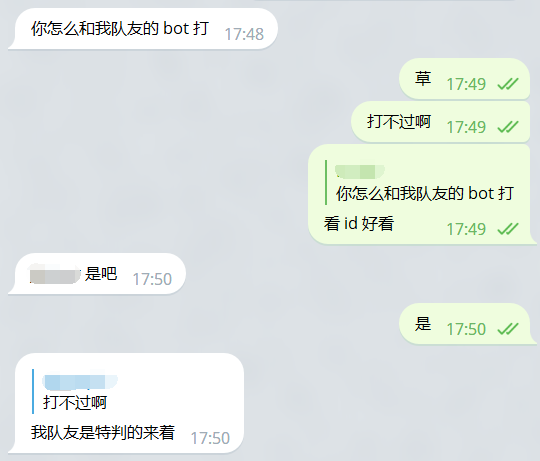
\includegraphics[width=6cm]{img/teammate.png}
		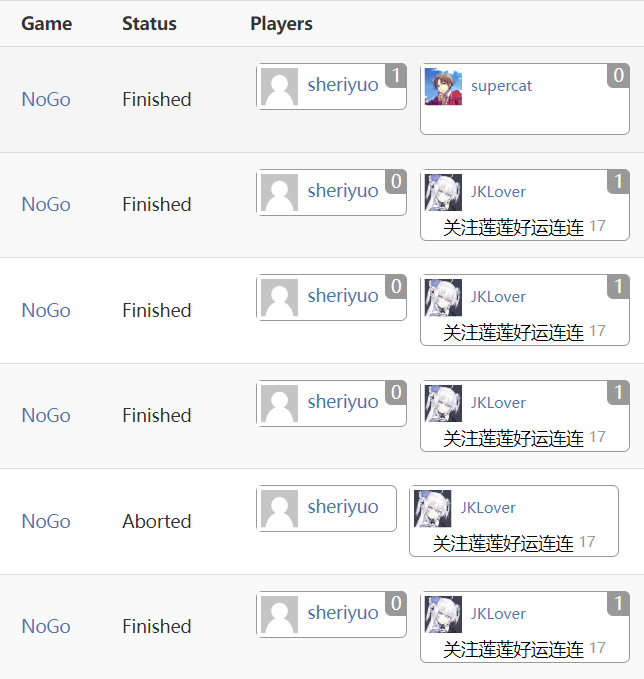
\includegraphics[width=6cm]{img/pk.png}
		
		\counterwithin{figure}{subsection}
		\caption{测试过程}
	\end{figure}
	
	同时由于 Minimax 搜索算法本身就不够优秀,所以与隔壁组的 MCTS 对战结果是打不过,合情合理。
	
	对于固定策略的 AI,对战结果可能与先后手相关性较强,该测试样本量较小,所以具体情况尚不明。理论上是因为固定策略会让估价函数有较大幅度的波动,对于调参造成了一定困难。
		
	\section{感谢}
	
	感谢孙亚辉老师、潘俊达助教在学习生活上的指导和关心。
	
	感谢中国人民大学图灵实验班提供交流的平台与机会。
	
	感谢冯友和、赵培宇同学组成的团队。
	
	感谢彭文博、李知非同学于 2023/3/2 军理课后请本队吃的 KFC 疯狂星期四,并日常交流立直麻将。
	
	感谢 rvalue 同学对冯友和同学提供的指导。
	
	感谢北京大学 glc 同学提供的帮助。
	
	感谢北京大学 Pecuria 同学提供的帮助。
	
	感谢北京大学 botzone 平台提供的 AI 对战支持。
	
	感谢雀魂麻将牌谱的设计参考。
	
\end{document}